\documentclass[11pt,a4paper]{article}
\usepackage[T1]{fontenc}
\usepackage[utf8]{inputenc}
\usepackage{lmodern}
\usepackage[margin=23mm,footskip=10mm]{geometry}
\usepackage{graphicx,xcolor,booktabs,tabularx,array,amsmath,fancyvrb}
\usepackage[pdfencoding=auto,psdextra]{hyperref}
\hypersetup{hidelinks,
  pdftitle={ActivityLink: On-device Activity Recognition and Data Availability Feedback},
  pdfsubject={Individual Internet of Things project, examination 17 November 2026},
  pdfauthor={Martina Speciale},pdfkeywords={IoT, MQTT, Contiki-NG, nRF52840, human activity recognition}}
\graphicspath{{assets-en/}}
\setlength{\parindent}{0pt}
\setlength{\parskip}{5pt}
\setlength{\emergencystretch}{2em}
\setlength{\tabcolsep}{5pt}
\renewcommand{\arraystretch}{1.15}
\setcounter{secnumdepth}{1}
\newcolumntype{Y}{>{\raggedright\arraybackslash}X}
\newcommand{\file}[1]{\nolinkurl{#1}}
\newcommand{\note}[1]{\par\smallskip{\small\itshape #1}\par\smallskip}
\newcommand{\reportsection}[1]{\section{#1}}
\newcommand{\sub}[1]{\subsection*{\normalsize #1}}
\DefineVerbatimEnvironment{Code}{Verbatim}{fontsize=\footnotesize,frame=none,xleftmargin=6pt}
\pagestyle{plain}
\begin{document}

\hypersetup{pageanchor=false}
\begin{titlepage}
\centering
\vspace*{8mm}

\includegraphics[width=65mm]{unipi-logo.pdf}\par
\vspace{10mm}
{\Large Internet of Things\par}
\vspace{7mm}
{\large Individual Project Report\par}
\vspace{18mm}
{\Huge\bfseries ActivityLink\par}
\vspace{8mm}
{\Large On-device activity recognition and\par
 data availability feedback\par}
\vspace{26mm}
{\small Martina Speciale\par}
\vspace{6mm}
{\small Student ID: 603047\par}
\vfill
{\large Examination: 17 November 2026\par}
\vspace{8mm}
{Technical report --- 4 November 2026\par}
\end{titlepage}
\hypersetup{pageanchor=true}
\pagenumbering{roman}
\tableofcontents
\clearpage
\pagenumbering{arabic}

\reportsection{Introduction}
ActivityLink demonstrates a small IoT system that classifies human activity on a microcontroller and displays both the activity category and the availability of recent data on a separate device. Movement is shown in green, posture in blue, and unavailable data in red. The Smart Health use case is a demonstration of daily activity monitoring; it does not provide clinical diagnoses or validated medical alerts.

Three real nRF52840 dongles implement the HAR node, the feedback actuator and the IPv6 border router. Sensing is simulated using precomputed UCI HAR feature vectors stored in flash. SVM inference and the HAR node's local LED decision run on the microcontroller. Moving the dongle does not change these stored inputs.

The Mac hosts Mosquitto, a Python backend, MySQL and Grafana. The backend persists validated telemetry and then reads SQL to choose the remote feedback command. This local deployment implements the role called the \emph{Cloud Application} in the project specification; no remote cloud service is used.

\begin{center}
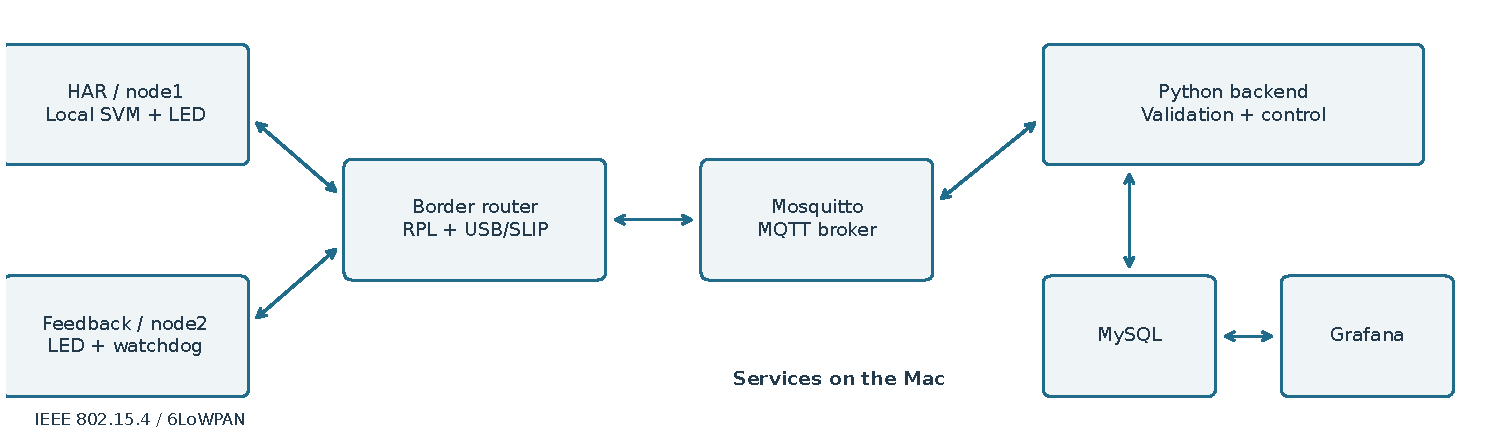
\includegraphics[width=\linewidth]{architecture.pdf}
\end{center}
{\small Communication links connect the radio network, the USB/SLIP border router and the services on the Mac. Grafana has read-only access to application data.}

\sub{One complete operating cycle}
\begin{enumerate}
\setlength{\itemsep}{0pt}
\setlength{\parskip}{0pt}
\item HAR selects a stored feature vector; the local SVM predicts its activity class and updates the local LED.
\item HAR publishes MQTT telemetry. The backend validates it and stores the accepted observation in MySQL.
\item The controller reads SQL, checks data freshness and publishes a feedback command; the actuator applies it and reports its state.
\item If HAR telemetry stops arriving, adaptive selects red once the last valid observation is older than six seconds. Fresh data restore activity feedback.
\end{enumerate}

The evaluation uses three paired adaptive/baseline trials, physical sensor disconnection and service recovery checks. The adaptation concerns \textbf{data freshness}: it changes the remote display when observations become obsolete; it does not retrain the SVM.

\clearpage
\reportsection{Devices, network and firmware}
\sub{Three physical roles}
\begin{tabularx}{\linewidth}{@{}l l Y@{}}
\toprule
Role & Observed USB port suffix & IPv6 address\\
\midrule
HAR / node1 & \texttt{E914240FC2B51} & \file{fd00::f6ce:3614:b5c2:f24}\\
Feedback / node2 & \texttt{E313BC9DEA181} & \file{fd00::f6ce:3613:18ea:9dbc}\\
Border router & \texttt{FA8130D5146E1} & \file{fd00::f6ce:3681:6e14:d530}\\
\bottomrule
\end{tabularx}

The border router connects the IEEE 802.15.4/6LoWPAN network to the Mac through SLIP over USB. Contiki's \texttt{tunslip6} configures \texttt{utun10} with \file{fd00::1/64}. Mosquitto listens on port 1883, including IPv6. RPL determines routing; the application design does not require every node to remain a direct radio child of the border router. Port identities are observations, not permanent role discovery.

\sub{Reproducible platform configuration}
Contiki-NG v5.1 is pinned to commit \file{2b87baf3ebdde3c8e37ca791d2bc84bfd76c49a4}. The application nodes use \texttt{TARGET=nrf BOARD=nrf52840/dongle}; the router uses \texttt{TARGET=nrf52840 BOARD=dongle}, as in the course laboratory. These are different Contiki platform implementations for the same SoC. The SW1 pin correction from P1.16 to P1.06 is included. The tested router uses the Nordic USB driver; an earlier TinyUSB FIFO experiment is not part of the deployed configuration.

The preserved 2 November images were compared with the binaries in the known DFU packages, filling unrecorded flash gaps with \texttt{0xff} where necessary. This is a file comparison, not a readback of device flash. Later source formatting and explicit configuration inclusion were checked by ARM compilation on 4 November; no new firmware was flashed during that regression.

\sub{Memory of the preserved images}
\begin{tabularx}{\linewidth}{@{}Yrr@{}}
\toprule
Role & HEX data bytes & Static RAM: .data + .bss\\
\midrule
HAR & 147,000 & 14,076 bytes\\
Feedback & 79,428 & 14,072 bytes\\
Border router & 80,192 & 13,840 bytes\\
\bottomrule
\end{tabularx}

{\small HEX data bytes exclude address gaps. The linker reserves 16,384 bytes each for stack and heap on application nodes, and 8,192/512 bytes on the router. These are reservations, not measured peak usage. Source: \file{results/2026-11-02-final/firmware/summary.json}.}

\sub{Local interaction and timing}
SW1 pauses/resumes HAR. During pause, activity and LED are zero but telemetry continues. SW1 on feedback toggles local LED mute while telemetry remains enabled. Button press changes state; release is only logged. A periodic application timer runs approximately every second. Connection attempts are separated by at least five seconds; the MQTT keepalive is 15 seconds and is managed by the MQTT library. Feedback turns red after more than eight seconds without a valid command, unless muted. The router can operate with its LEDs off.

\clearpage
\reportsection{On-device machine learning}
\sub{Dataset and subject separation}
UCI Human Activity Recognition Using Smartphones contains six activities from 30 volunteers [2]. The official split contains 7,352 training windows and 2,947 test windows from disjoint subjects. Each input has 561 precomputed features. Raw-signal acquisition and feature extraction are not implemented on the dongle.

The fixed recipe is \texttt{StandardScaler} followed by \texttt{LinearSVC(C=0.1)}, using six one-versus-rest linear scores. The current trainer reads only the official training files. Five-fold \texttt{GroupKFold} separates people between training and validation. A fresh scaler and classifier are fitted inside each fold; each training row receives one out-of-fold (OOF) prediction. No hyperparameter search or test-based acceptance rule is applied.

\sub{Export and execution}
After fitting the fixed recipe on training data, standardization is folded into the linear coefficients:
\[
 w'_{ji}=\frac{w_{ji}}{\sigma_i},\qquad
 b'_j=b_j-\sum_i w'_{ji}\mu_i,\qquad
 \hat y=\operatorname*{arg\,max}_j\left(b'_j+\sum_i w'_{ji}x_i\right).
\]
The firmware uses float32 parameters and chooses the largest of six scores. These scores are not probabilities. The 24 demonstration vectors (four per class) cycle through flash at approximately 1 Hz. Classes 1--3 represent movement and map to green; classes 4--6 represent sitting, standing and lying, and map to blue. Only the predicted class and node state are transmitted, not all feature values.

\begin{tabularx}{\linewidth}{@{}Yr@{}}
\toprule
Validation or implementation check & Result\\
\midrule
\textbf{Training-only subject-grouped OOF macro-F1} & \textbf{93.66\%}\\
OOF accuracy & 93.77\%\\
Fold macro-F1 range & 89.09--98.68\%\\
Fold macro-F1 standard deviation & 4.03 percentage points\\
Python/C prediction disagreements on 2,947 test inputs & 0\\
HAR inference observed on 15 device samples & 1.152--1.168 ms\\
\bottomrule
\end{tabularx}

The timing measurement covers only inference: 72--73 RTIMER ticks at 62,500 ticks/s. It excludes radio, backend work and feature extraction, and is not a worst-case execution-time bound. Python/C equivalence was checked on the host compiler; it does not mean 100\% classification accuracy or execution of all 2,947 windows on ARM.

\sub{Historical benchmark and limits}
The already-consulted official test gives historical accuracy 96.1995\% and macro-F1 96.2914\%. It is retained for traceability, not used to select the current candidate. Training isolation does not undo earlier consultation: an independent external confirmation would require previously unseen data. The notebook runs locally with Python 3.13, NumPy 2.3.5 and scikit-learn 1.8.0; hosted Colab execution has not been verified. Firmware export uses the frozen reference; retraining does not automatically replace it. The 24 demonstration vectors are not an accuracy study.

\clearpage
\reportsection{Messaging, persistence and control}
\sub{Why MQTT and JSON}
MQTT separates telemetry producers, the controller and observers through named topics. Its publish/subscribe model suits periodic updates and commands, with clients available in Contiki and Python. Mosquitto hosts the broker; Python uses Eclipse Paho. JSON makes telemetry inspectable and supports explicit field/type validation. This choice does not imply a measured performance advantage over CoAP.

MQTT 3.1.1 uses clean sessions, QoS 0 and non-retained messages. QoS 0 avoids per-message acknowledgment overhead but permits loss. Non-retained commands prevent automatic replay of an old command on reconnection. Repeated fresh commands and the local feedback watchdog support recovery.

\sub{Message contract}
\begin{Code}
activitylink/node1/telemetry
{"node":"node1","boot":"0123456789abcdef","seq":12,
 "uptime":20,"activity":1,"enabled":1,"led":1}
\end{Code}
Feedback publishes the same fields under \file{activitylink/node2/telemetry}, with activity 0 and enabled 1. The CLI publishes ASCII \texttt{P}/\texttt{R} to \file{activitylink/node1/command}; the controller publishes \texttt{0}--\texttt{3} to \file{activitylink/node2/command}. Commands are one byte. The firmware buffer is 240 bytes; the backend rejects payloads above 512 bytes, invalid UTF-8/JSON, repeated or unexpected fields, wrong types, incoherent node/topic or activity/LED values, and retained telemetry.

\sub{Database structure and control}
{\small
\begin{tabularx}{\linewidth}{@{}lYY@{}}
\toprule
Table & Key and stored observations & Purpose\\
\midrule
\texttt{telemetry} & Composite key \texttt{(node, boot, seq)}; reception time, uptime, activity, enabled and LED & Accepted device data read by the controller\\
\texttt{metrics} & Primary key \texttt{id}; time, run, mode, stale flags, command/reported LED and counters & Backend observations read by Grafana\\
\bottomrule
\end{tabularx}}

Duplicates and lower sequence numbers do not refresh observations; a new boot permits sequence restart. The controller reads the latest accepted rows about once per second. Roles are static in \file{config/devices.json}. Sensor data are stale when missing or older than six seconds since reception; this is not radio one-way latency.

\begin{tabularx}{\linewidth}{@{}YYY@{}}
\toprule
Condition & Adaptive & Baseline\\
\midrule
No sensor row & Red & Red\\
Stale sensor row & Red & Keep last activity or pause\\
Fresh pause & Off & Off\\
Fresh movement/posture & Green/blue & Green/blue\\
\bottomrule
\end{tabularx}

Callbacks feed a 1,000-item RAM queue; SQL errors retain the pending item for retry. The queue is lost on restart. Grafana reads SQL in UTC; counters are cumulative per backend process. A reported LED of $-1$ means missing/stale feedback. The boot ID is not cryptographic identity. The lab broker has no TLS/authentication; MySQL and Grafana bind to localhost.

\clearpage
\reportsection{Experimental design}
\sub{Required individual-project stress scenario}
The specification requires faulty/intermittent-node evaluation and an adaptive mechanism compared with adaptation disabled [1]. The experiment uses real dongles, IPv6/RPL, Mosquitto, SQL and the feedback actuator. A temporary relay broker on \texttt{localhost:18884} forwards original telemetry and actuator commands, withholding only HAR telemetry during a controlled fault window.

Each run lasts 40 seconds: 10 normal, 15 with selective loss, and 15 of recovery. Three adaptive/baseline pairs alternate execution order. The ordinary backend is stopped during the experiment and restored afterward; no simulator uses the real device IDs concurrently.

\note{Fault injection is at \textbf{backend ingress}. HAR continues classifying and transmitting over the radio. This experiment isolates the control response to missing data; it does not measure radio packet-delivery ratio, radio congestion or a physical power failure. Physical unplug/replug is a separate check.}

\sub{Measurements and traceability}
\file{wire.jsonl} records observed messages and intentional drops. Per-run \file{metrics.json} stores SQL decisions and counters. Detection time runs from the last forwarded sensor message to the first stale controller sample. Reported LED behavior is evaluated in a stabilized window beginning at +19 s, allowing time for detection, command propagation and reporting.

\begin{tabularx}{\linewidth}{@{}Yrrrrc@{}}
\toprule
Mode & Drops & Stale & Red/stale & Detect (s) & Recovery\\
\midrule
Adaptive & 15 & 9 & 9/9 & 6.816 & Yes\\
Baseline & 14 & 9 & 0/9 & 6.381 & Yes\\
Baseline & 15 & 9 & 0/9 & 6.340 & Yes\\
Adaptive & 15 & 10 & 10/10 & 6.015 & Yes\\
Adaptive & 15 & 9 & 9/9 & 6.933 & Yes\\
Baseline & 15 & 9 & 0/9 & 6.045 & Yes\\
\bottomrule
\end{tabularx}

Rows follow execution order. Equal fault durations do not imply identical message counts or activity traces: transmission phase and cyclic inputs differ. The first adaptive run is not paired with an identical sequence of activity changes. No statistical significance or broad deployment generality is claimed from three short pairs.

\sub{Additional acceptance checks}
A passive hardware capture collected 100 valid JSON messages per node in 100 seconds without observed sequence gaps. Other checks cover pause/resume propagation through SQL, LED commands, physical buttons, watchdog behavior, duplicate/out-of-order handling and recovery. The latest regression on 4 November verifies the renamed backend commands and the readable CLI against real dongles. Evidence from hardware, simulations and mocked unit tests is kept separate.

{\small Sources: \file{results/2026-11-02-final/stress/summary.json} and per-run measurements;\\
latest regression: \file{results/2026-11-04-hardware-regression/}.}

\clearpage
\reportsection{Adaptive/baseline results}
Across the six runs, adaptive selects red for \textbf{28/28 stale controller samples}; baseline selects red for \textbf{0/27}. In the stabilized actuator window, reported red occurs in \textbf{17/17} adaptive reports versus \textbf{0/17} baseline reports. All six runs recover after forwarding resumes. Final validation and queue-overflow counters remain zero in these trials.

\noindent\makebox[\linewidth][c]{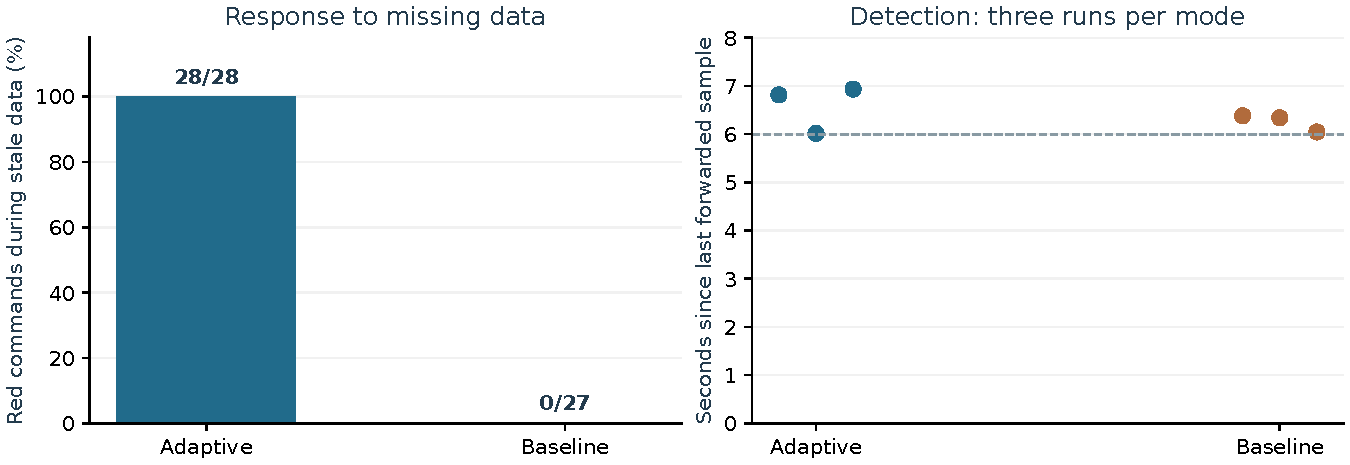
\includegraphics[width=0.90\linewidth,height=37mm,keepaspectratio]{stress-comparison.pdf}}\par
{\small\textbf{Figure 1.} Aggregate response and detection time. Each dot is one run; the dashed line marks the nominal six-second stale threshold.}

\smallskip
\noindent\textbf{Adaptive: missing telemetry triggers red feedback}\par
\noindent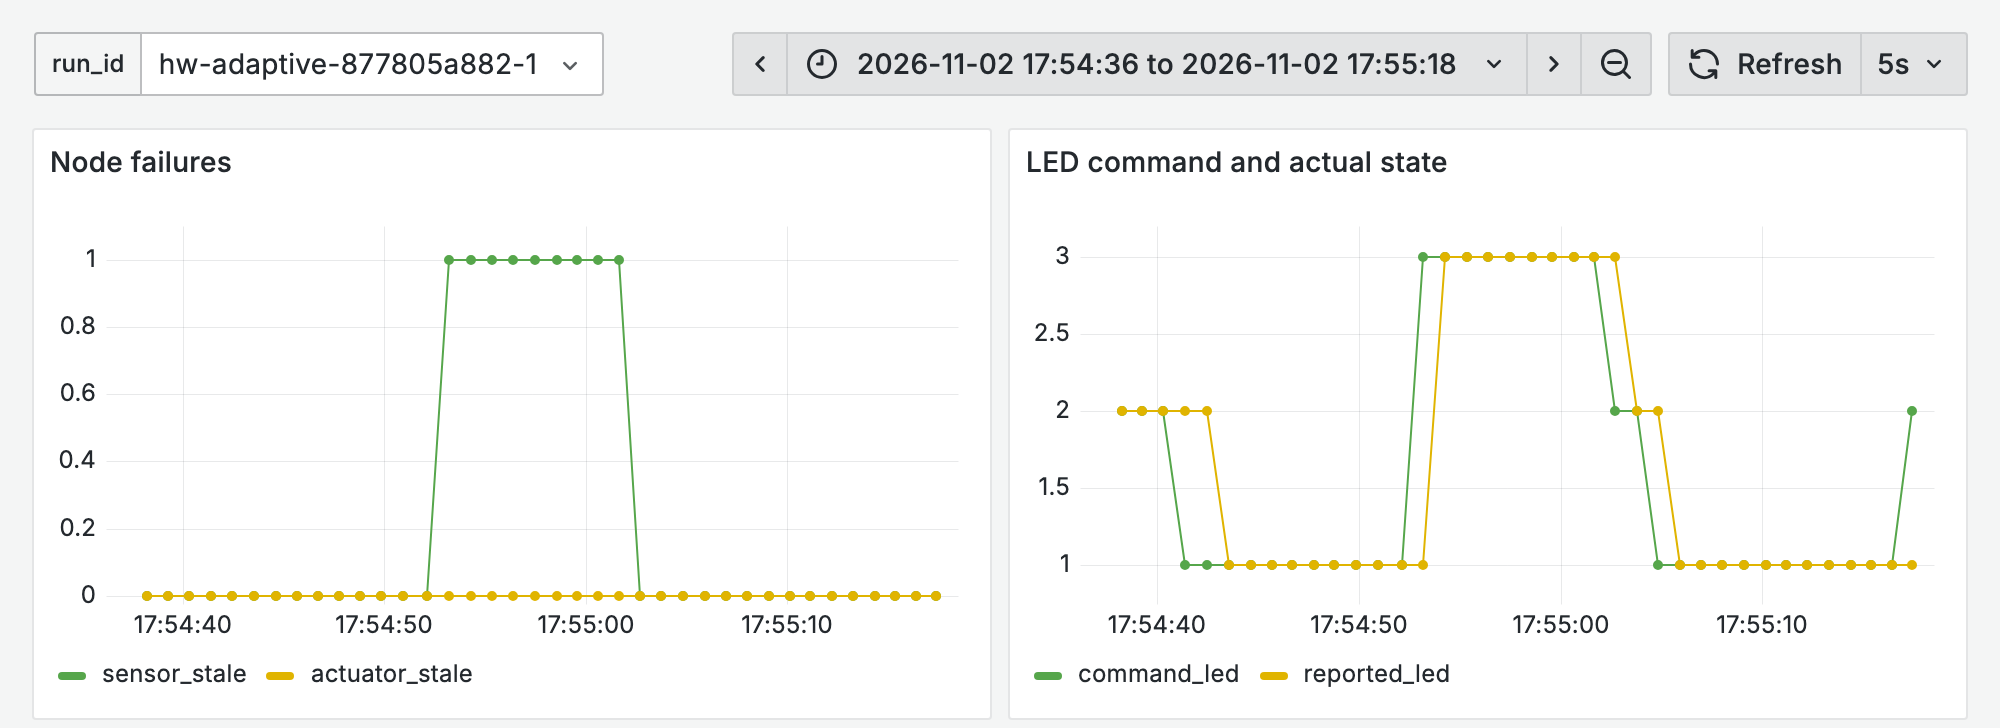
\includegraphics[width=\linewidth]{grafana-adaptive.png}\par
\noindent\textbf{Baseline: the last activity remains displayed}\par
\noindent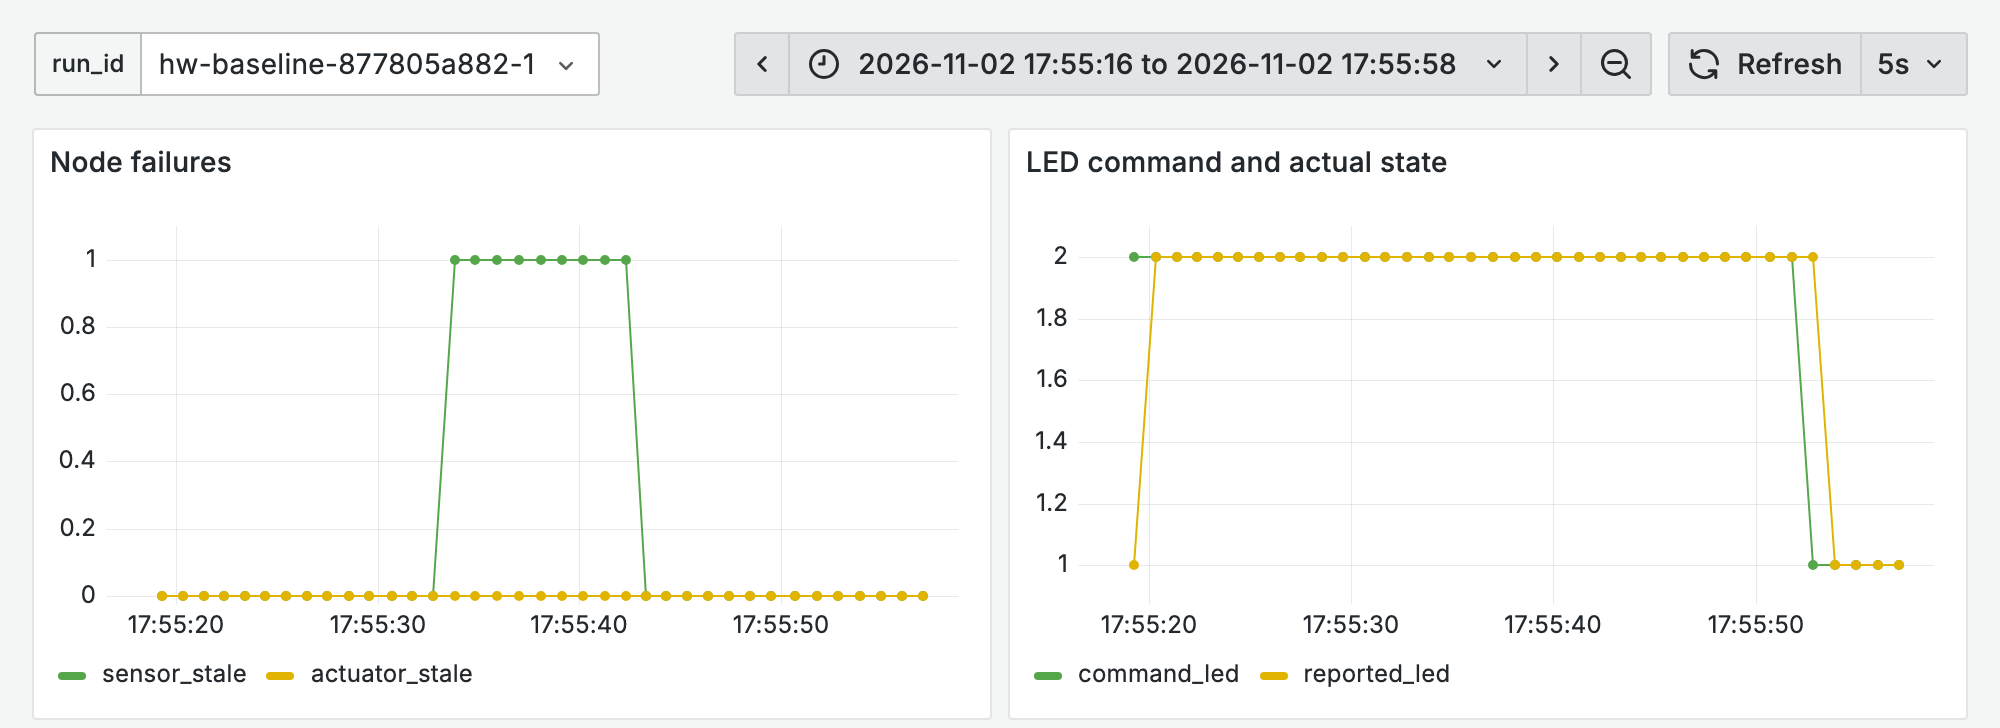
\includegraphics[width=\linewidth]{grafana-baseline.png}\par
{\small\textbf{Figure 2.} Real Grafana views captured on 4 November from the 2 November hardware runs. Left: sensor stale rises to 1; actuator stale stays 0. Right: adaptive selects red (3), while baseline retains blue (2); reports can lag commands. Both recover. Codes: 0 off, 1 green, 2 blue, 3 red. Activity sequences differ. Both modes use the same detector; adaptation changes the response. Images and capture metadata are supplied; these are archived measurements, not new experiments.}

\clearpage
\reportsection{Robustness and latest regression}
\sub{Physical disconnection and service recovery}
A separate test unplugged HAR while leaving router and feedback connected. The system recorded sensor stale and red feedback, then accepted a new HAR boot and returned to activity feedback after reconnection. The user confirmed recovery. RPL reconvergence latency is not estimated because the physical reinsertion timestamp was not recorded precisely.

\begin{tabularx}{\linewidth}{@{}lY@{}}
\toprule
Check & Verified observation\\
\midrule
MySQL unavailable & Local feedback watchdog turns red; backend process survives\\
MySQL recovery & All 35 messages observed during the outage are later present in SQL\\
Broker restart & Automatic recovery observed 6.81 s after broker startup\\
SQL contract & Insert, duplicate, ordering, reboot and freshness checks pass\\
4 November regression & Real pause/resume, backend stop/restart and four Grafana panel queries pass\\
Current unit suite & 10 backend/protocol tests and 2 ML-isolation tests pass\\
\bottomrule
\end{tabularx}

During SQL failure, buffered messages retain their original receive times. During broker failure, QoS 0 can lose telemetry: the criterion is recovery to fresh data and coherent feedback, not guaranteed replay of every missed packet.

\sub{Additional queue saturation check}
Saturating the queue is not an explicit individual-project requirement, but the full-queue branch was tested separately. The real backend callback receives a burst of 1,005 valid messages before consumption: 1,000 are queued and five rejected. After one simulated SQL connection error, the processing loop drains the first 1,000 in FIFO order and reports accepted=1,000 and queue drops=5.

MQTT and SQL are replaced by test objects in this check; storage calls are observed rather than written to real MySQL. It verifies queue capacity, overflow counting and recovery of consumption, not radio performance or real SQL throughput. Earlier hardware runs with zero queue drops did not exercise saturation.

\sub{Interpretation and limitations}
The 4 November hardware regression exercises the current Python CLI and \texttt{stop-backend} and \texttt{start-backend}: stopping the backend leaves broker, SQL and Grafana active, feedback reports watchdog red, and restarting restores control. Reported LED codes are device software observations, not optical measurements. No new flash or retraining was needed.

The evaluation covers one three-dongle setup and short trials. It does not establish energy consumption, peak RAM, radio PDR, congestion behavior, clinical accuracy or long-term reliability. The official ML test is historical; hosted Colab remains unverified. Detailed additional evidence is in \file{docs/QUEUE_SATURATION_CHECK.md} and the dated regression directories.

\clearpage
\reportsection{Conclusions and reproduction}
\sub{What the experiments establish}
ActivityLink integrates on-device activity classification, MQTT telemetry, SQL-based control and a separate feedback actuator on a three-dongle network. The stored feature vectors simulate sensing; classification and the local activity decision execute on HAR. The backend then combines the activity with data freshness to control the remote display.

The key result is a change in behavior when observations become obsolete. Across three runs per mode, adaptive selects red for 28/28 stale controller samples, while baseline selects red for 0/27. Both modes detect the same stale condition; adaptation changes the response rather than accelerating detection. The stabilized actuator reports support the command-level result, and all six trials recover after telemetry forwarding resumes.

This distinction matters for the demonstration: a displayed activity should not silently imply a recent observation when the sensor is unavailable. The red indication expresses unavailable data, not a health diagnosis. Physical disconnection and service recovery checks complement the controlled-loss experiment; the mocked queue check exercises a separate software failure path.

\sub{Scope and next steps}
The evidence concerns one small deployment and short experiments. It does not establish clinical accuracy, radio packet delivery ratio, energy efficiency or long-term reliability. The ML out-of-fold evaluation separates training subjects; the previously consulted official test remains a historical benchmark. Neither the 24 embedded examples nor successful control recovery establish accuracy for live patient monitoring.

A further evaluation would require previously unseen subjects, longer and repeated outages, and real sensor acquisition with a compatible feature-extraction pipeline. Such measurements would extend the evidence; they are not claimed as completed work.

\sub{Reproducing the demonstrated configuration}
Complete setup, build, startup and shutdown commands are in \file{README.md}, \file{docs/REPRODUCE.md} and \file{docs/NATIVE_MAC_STACK.md}. The prepared Mac uses Contiki's original \texttt{connect-router} target and the Python CLI. Local credentials and service databases are excluded.

Grafana is at \url{http://127.0.0.1:3000/d/activitylink}. Select an archived \texttt{run\_id} and its recorded interval using the supplied summaries and screenshot metadata. Report compilation uses the supplied figures; it requires neither dongles nor new experiments.

\sub{References}
{\footnotesize\raggedright
[1] Course specification, \emph{IoT Project 2026}, pp. 1--3; \emph{Righetti laboratory slides}, pp. 7, 12, 75, 90 and 193. Local teaching material is not redistributed.\\[3pt]
[2] Reyes-Ortiz et al., \emph{Human Activity Recognition Using Smartphones}, UCI Machine Learning Repository (2013). \url{https://doi.org/10.24432/C54S4K}. CC BY 4.0; attribution in \file{data/ATTRIBUTION.md}.\\[3pt]
[3] \href{https://github.com/contiki-ng/contiki-ng}{Contiki-NG source repository}, pinned v5.1 revision; platform definitions and MQTT implementation in the retrieved sources.\\[3pt]
[4] \href{https://mosquitto.org/}{Eclipse Mosquitto} 2.0.22 and \href{https://eclipse.dev/paho/clients/python/docs/}{Eclipse Paho MQTT Python client}. Component notices are in \file{THIRD_PARTY.md}.\\[3pt]
[5] \href{https://grafana.com/docs/grafana/latest/datasources/mysql/}{Grafana MySQL datasource documentation}. Tested native versions: Grafana 11.6.0 and MySQL Community 8.0.31 on macOS 12 Intel.
}
\end{document}
